\chapter{Singleton模式}
\section{单例模式的概念}
\subsection{定义}
单例(Singleton)模式的定义:指一个类只有一个实例,且该类能自行创建这个实例的一种模式。
\subsection{特点}
\begin{enumerate}
	\item 单例类只有一个实例对象;
	\item 该单例对象必须由单例类自行创建;
	\item 单例类对外提供一个访问该单例的全局访问点;
	\item 构造函数为private,避免自行创建实例;
\end{enumerate}
\subsection{优点}
\begin{enumerate}
	\item 由于单例模式在内存中只有一个实例,减少内存开支,特别是一个对象需要频繁地创建销毁时,而且创建或销毁时性能又无法优化,单例模式就非常明显了;
	\item 由于单例模式只生成一个实例,所以,减少系统的性能开销;
	\item 单例模式可以避免对资源的多重占用,例如一个写文件操作,由于只有一个实例存在内存中,避免对同一个资源文件的同时写操作
	\item 单例模式可以在系统设置全局的访问点,优化和共享资源访问,例如,可以设计一个单例类,负责所有数据表的映射处理。
\end{enumerate}
\subsection{缺点}
\begin{enumerate}
	\item 单例模式没有抽象层,扩展很困难,若要扩展,除了修改代码基本上没有第二种途径可以实现;
	\item 单例类的职责过重,在一定程度上违背了“单一职责原则”;
	\item 滥用单例将带来一些负面问题,如:为了节省资源将数据库连接池对象设计为的单例类,可能会导致共享连接池对象的程序过多而出现连接池溢出;
\end{enumerate}
\subsection{角色}
\begin{itemize}
	\item Singleton: 返回唯一实例static方法;
	\item 访问类:客户端使用Singleton的getInstance()方法。
\end{itemize}
\subsection{应用场景}
\begin{enumerate}
	\item 当某类需要频繁实例化,而创建的对象又频繁被销毁的时候,如多线程的线程池、网络连接池等;
	\item 在应用场景中,某类只要求生成一个对象的时候。
\end{enumerate}
\subsection{模式框架图}
\begin{figure}[!h]
	\centering
	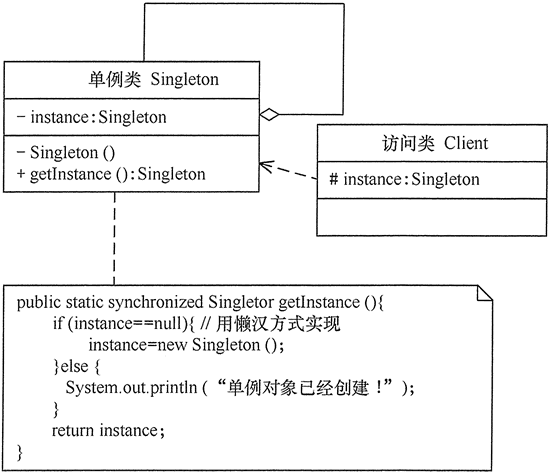
\includegraphics[width=0.8\textwidth]{image/5-1}
	\caption{单例模式的结构图}
\end{figure}
\section{饿汉模式}
通常,普通类的构造函数是公有的,外部类可以通过“new 构造函数()”来生成多个实例。但是,如果将类的构造函数设为私有的,外部类就无法调用该构造函数,也就无法生成多个实例。这时该类自身必须定义一个静态私有实例,并向外提供一个静态的公有函数用于创建或获取该静态私有实例。
\begin{lstlisting}
public class Singleton {
	private static Singleton singleton = new Singleton();
	private Singleton() {
		System.out.println("New a instance");
	}
	public static Singleton getInstance() {
		return singleton;
	}
}
public class Main {
	public static void main(String[] args) {
		System.out.println("Satrt:");
		Singleton obj1 = Singleton.getInstance();
		Singleton obj2 = Singleton.getInstance();
		if (obj1 == obj2) {
			System.out.println("Equal");
		} else {
			System.out.println("Not equal");
		}
		System.out.println("End.");
	}
}
\end{lstlisting}
\begin{lstlisting}
//output
Satrt:
New a instance
Equal
End.
\end{lstlisting}
\section{多线程懒汉模式}
如果编写的是多线程程序,则不要删除上例代码中的关键字 volatile 和 synchronized,否则将存在线程非安全的问题。如果不删除这两个关键字就能保证线程安全,但是每次访问时都要同步,会影响性能,且消耗更多的资源,这是懒汉式单例的缺点。
\begin{lstlisting}
public class LazySingleton {
	//保证 instance 在所有线程中同步
	private static volatile LazySingleton instance = null;
	//private 避免类在外部被实例化
	private LazySingleton() {
	}
	//getInstance 方法前加同步
	public static synchronized LazySingleton getInstance() {
		if (instance == null) {
			instance = new LazySingleton();
		}
		return instance;
	}
}
\end{lstlisting}
\section{模式扩展——多例模式}
\begin{figure}[!h]
	\centering
	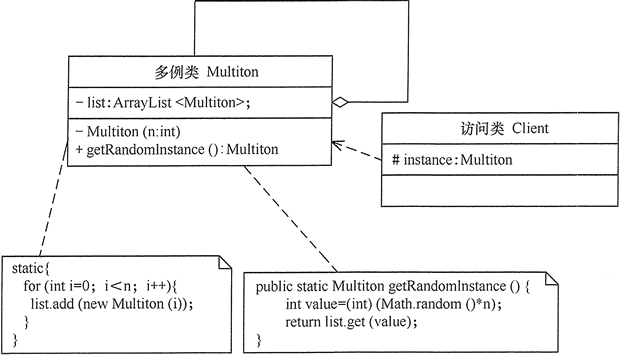
\includegraphics[width=0.8\textwidth]{image/5-2}
	\caption{有限的多例模式的结构图}
\end{figure}
\section{不严格的Singleton}
下面是不严格的单例模式,多线程可能会生成多个实例。
\begin{lstlisting}
public class Singleton {
	private static Singleton singleton = null;
	private Singleton() {
		System.out.println("New a instance");
	}
	public static Singleton getInstance() {
		if (singleton == null) {
			singleton = new Singleton();
		}
		return singleton;
	}
}
\end{lstlisting}
\par 可以参照多线程饿汉模式加上关键字synchronized即可。